\chapter{Informationstheorie}
\index{Informationstheorie|(}
\section{Information und Entropie}
\index{Information und Entropie|(}

\begin{bsp}Aus einem Stoß mit 16 Schnapskarten zieht Spieler A zufällig eine Karte, 
Spieler B stellt nun Fragen über die Karte, die A mit "ja" oder "nein" beantworten darf.\\
Wie viele Fragen sind (bei optimaler Spielweise) maximal notwendig, um die zufällig gezogene Karte zu erraten?
\end{bsp}

Mit der optimalen Strategie, der binäre Suche (Menge der noch möglichen Karten in gleichgroße disjunkte Teilmengen aufspalten und Fragen ob x in der ersten Teilmenge enthalten ist), lässt sich die maximale Spieldauer bestimmen:

Da wir wissen, dass unsere Schnapskarte X mit einer diskreten Gleichverteilung $p_x = \frac{1}{16}$ verteilt ist, können wir ihren Informationsgehalt bestimmen:
\begin{definition}[Informationsgehalt]\index{Informationsgehalt}
Der Informationsgehalt \gls{symb:I} einer Zufallsvariable X mit der Wahrscheinlichkeit $p_x$ ist definiert als:\\
\begin{align}
I_x = I(p_x) = log_2(\frac{1}{p_x}) = - log_2(p_x)
\end{align}

\end{definition}
Ergibt in unserem Fall\\
$I_x = log_2(16) = 4 \dots $ bit (ja-nein Fragen)\\

Interessanter wird es, wenn Spieler A die Karte nicht mehr zieht, sondern zufällig mit der Verteilung $P=(p_1,\dots, p_m)$
wählt.\\
Da die Wahrscheinlichkeiten der Karten jetzt nicht mehr alle gleich sind und wir somit die Wahrscheinlichkeit der verdeckten Karte nicht kennen, können wir nicht so einfach den Informationsgehalt der gewählten Karte bestimmen.\\

Da wir jedoch die Verteilung $P$ kennen, können wir damit den \textbf{mittleren Informationsgehalt} bzw. die 
\textbf{Informationsdichte} bestimmten:\\
\begin{definition}[Entropie]\index{Entropie}
Die Entropie \gls{symb:H} ist ein Maß für den mittleren Informationsgehalt bzw. der Informationsdichte einer Verteilung.\\
Sie ist definiert als \textbf{Erwartungswert} des Informationsgehalts:
\begin{align}
H(P) = \sum_{i=1}^{m}I(p_i) = - \sum_{i=1}^{m}p_i log_2(p_i)
\end{align}
Für eine Zufallsvariable $X \sim P$ gilt:
\begin{align}
H(X) = H(P)
\end{align}
\end{definition}

In unserem Spiel müssen jetzt eine neue Strategie finden, da die einfache binäre Suche nicht mehr eindeutig definiert ist.\\
Eine Strategie kann als Binärbaum dargestellt werden und umgekehrt repräsentiert ein Binärbaum eine Spielstrategie:\\
Jeder innere Knoten entspricht einer Frage, jede linke ausgehende Kante einer Antwort "ja" und jede rechte ausgehende Kante einem "nein". Die Endknoten (Blätter) stellen einen Wert X der Zufallsvariable dar.\\
Es gibt genau \gls{symb:m}-Blätter, denn es existieren ja auch $m$ Zufallsvariablen.
Beispiel mit $x ~ \lbrace 1, 2, 3, 4 \rbrace$:\\
\begin{center}
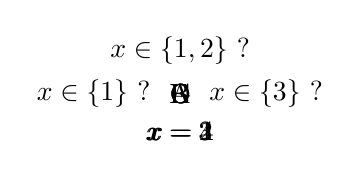
\begin{tikzpicture}[every tree node/.style={draw,circle},
   level distance=1.25cm,sibling distance=.5cm, anchor=west,
   edge from parent path={(\tikzparentnode) -- (\tikzchildnode)}]
%  \tikzstyle{level 1}=[sibling distance=60mm]
%  \tikzstyle{level 2}=[sibling distance=30mm]
%  \tikzstyle{level 3}=[sibling distance=60mm]
%\node {$x \in \lbrace 1, 2 \rbrace$ ?}
%	child {node {$x \in \lbrace 1 \rbrace$ ?}
%		child{node {x=1}} 
%		child{node {x=2}}
%	}
%	child {node  {$x \in \lbrace 3 \rbrace$ ?}
%			child{node  {x=3}}
%			child{node {x=4}}
%	};
	\Tree [.\node[label=north: {$x \in \lbrace 1, 2 \rbrace$ ?}] (A) {A} ; 
	  \edge node[auto=right] {\textcolor{blue}{"ja"}};  
	    [.\node[label=west: {$x \in \lbrace 1 \rbrace$ ?}] (B) {B};  
	      [.\node[label=south: {$x = 1$}] (D) {D};  ] [.\node[label=south: {$x = 2$}] (E) {E}; ]
	    ]
	  \edge node[auto=left] {\textcolor{blue}{"nein"}};  
	    [.\node[label=east: {$x \in \lbrace 3 \rbrace$ ?}] (C) {C}; 
	     [.\node[label=south: {$x = 3$}] (F) {F};  ] [.\node[label=south: {$x = 4$}] (G) {G}; ]
	    ] ]
\end{tikzpicture}
\end{center}


Die Suche nach der
optimalen Strategie lässt sich so formulieren, dass wir unter
allen Binärbäumen denjenigen suchen, für den \textbf{mittlere Unbestimmtheit} minimal ist:

\begin{definition}[Mittlere Unbestimmtheit]\index{Mittlere Unbestimmtheit}\index{Mittlere Codewortlänge|see{Mittlere Unbestimmtheit}}\index{Codewortlänge!Mittlere-|see{Mittlere Unbestimmtheit}}\index{Mittlere Blattlänge|see{Mittlere Unbestimmtheit}}\index{Blattlänge!Mittlere-|see{Mittlere Unbestimmtheit}}\index{Unbestimmtheit!Mittlere-|see{Mittlere Unbestimmtheit}}\label{def:mittlere_unbestimmtheit}
Als mittlere Unbestimmtheit \gls{symb:Hstar} bzw. mittlere Codewortlänge oder auch mittlere Blattlänge definiert ist:
\begin{align}
H^*(P) = \sum_{i=1}^{m} p_i l_i
\end{align}
wobei $l_i$ die Blattlänge des Blatts mit dem Index $i$ (also seine Entfernung von der Wurzel)
\end{definition}

Für diese Aufgabe
ist es nützlich zu wissen, wann ein Binärbaum mit den 
Blattlängen $l_1,\dots l_m$ existiert.
\begin{satz}[Ungleichung von Kraft]\index{Ungleichung!von Kraft}\index{Kraft Ungleichung|see{Ungleichung von Kraft}}
Ein Binärbaum mit den Blattlängen $L_1,\dots,l_m$ existiert genau dann,
wenn 
\[\sum_{i=1}^m2^{-l_i}\le 1.\]
Gleichheit gilt genau dann, wenn der Baum vollständig ist.
\end{satz}

Die Suche nach der optimalen Strategie besteht also darin,
\[\sum p_il_i\]
unter der Nebenbedingung
\[\sum 2^{-l_i}\le 1\]
zu minimieren. Es ist leicht einzusehen, dass im optimalen Fall in der
letzten Ungleichung Gleichheit gelten muss (sonst könnten wir einfach 
dass größte $l_i$ verkleinern).
Wenn wir die Forderung, dass $l_i$ ganzzahlig sein muss, beiseite lassen,
lässt sich das Minimum mit der Lagrange-Methode bestimmen  und hat den Wert
\[\sum p_i\log_2(\frac{1}{p_i}).\]
Dies entspricht der \textbf{Entropie}, die minimale Spieldauer bei optimaler Strategie ist also durch die Entropie bestimmt.\\

\begin{definition}[Huffman-Algorithmus]\label{def:huffman_algorithmus}
Die optimale Spielweise für eine Verteilung $P=(p_1,\dots, p_m)$ ist der sogenannte \textbf{Huffman-Algorithmus}\index{Huffman-Algorithmus}\index{Algorithmus!Huffman|see{Huffman Algorithmus}}, der folgendermaßen vorgeht:

\begin{enumerate}
\item Wenn $m=1$, dann besteht der Baum nur aus der Wurzel, Ende.
\item Ordne die Wahrscheinlichkeiten: $p_1\ge\dots\ge p_m$.
\item Fasse die zwei kleinsten Wahrscheinlichkeiten zusammen: 
$p^*_{m-1}=p_{m-1}+p_m$,
\item Konstruiere den optimalen Baum für $P^*=(p_2,\dots,p_{m-1},p_{m-2}^*)$
\item Ersetze Blatt $m-1$ durch einen inneren Knoten mit den Blättern
$m-1$ und $m$.
\end{enumerate}
\end{definition}
Für den Huffman-Algorithmus gilt:
\begin{satz} %gilt nur bei Huffman
$H(P) \leq H^*(P) \leq H(P) +1$
\end{satz}

Der Summand 1 in der oberen Abschätzung stört ein wenig; man kann
diese Differenz verringern, indem man statt eines einzelnen
Elements mehrere (unabhängige und identisch verteilte) errät, sagen wir $n$.
Die Entropie der gemeinsamen Verteilung ist (wie weiter unten
gezeigt wird) Entropie $nH(P)$, damit lässt sich die mittlere Anzahl der
Fragen, um den gesamten Block zu erraten, mit $nH(P)+1$
abschätzen, pro Element ergibt das $H(P)+1/n$, was beliebig nahe an
die Entropie herankommt.


\subsection{Bedingte Entropie und die Kullback-Leibler Divergenz}
Wenn $X$ und $Y$ zwei Zufallsvariable sind, können wir $(X,Y)$
als eine neue Zufallsvariable mit Wahrscheinlichkeit $p(x, y)=\mathbb P(X=x, Y=y)$ betrachten.\\
Die Entropie, die diese neuen Zufallsvariable besitzt, heißt  \textbf{gemeinsame Entropie} von X und Y:\index{gemeinsame Entropie}\index{Entropie!gemeinsame-|see{gemeinsame Entropie}}\\
 \[H(X,Y)=H((X,Y))\]
Nehmen wir die bedingte Wahrscheinlichkeit
$p(x|y)=\mathbb P(X=x|Y=y)$ und definieren
\begin{definition}[Bedingte Entropie]\index{Bedingte Entropie}\index{Entropie!Bedingte-|see{Bedingte Entropie}}
\[H(X|Y=y)=-\sum_x p(x|y)\log_2(p(x|y))\]
und nennen
\[H(X|Y)=\sum_x p_Y(y)H(X|Y=y)\]
die \textbf{bedingte Entropie} von $X$ unter $Y$.
\end{definition}
Die bedingte Entropie ist ein Maß für die "Ungewissheit" die über einer Variable (X) verbleibt, wenn eine andere Variable (Y) bekannt ist.\\

Der Wertebereich für die bedingte Entropie ist folgendermaßen beschränkt:

\[ 0 \le H(X|Y) \le H(X)\]

Genauer gilt:
\begin{satz}
\[H(X|Y) = H(X)\]
falls X und Y stochastisch unabhängig sind und
\[H(X|Y) = 0\]
falls X aus Y funktionell bestimmt werden kann, das heißt es existiert eine Funktion $g$ mit $X = g(Y)$
\end{satz}
Aus diesem Satz ergeben sich weitere Eigenschaften für die \textbf{bedingte} bzw. die \textbf{gemeinsame Entropie}.\index{Bedingte Entropie}\index{gemeinsame Entropie}
\begin{satz}
\[H(X,Y)=H(Y)+H(X|Y),\]
\[\max(H(X),H(Y))\le H(X,Y)\le H(X)+H(Y),`\]
\[H(X|Y)\le H(X),\]
\[H(X|Y,Z)\le H(X|Y).\]
\[H(X,Y)=H(X)+H(Y)\]
gilt genau dann, wenn $X$ und $Y$ unabhängig sind.
\[H(X,Y)=H(X)\]
gilt genau dann, wenn es eine Funktion $g$ gibt, sodass $Y=g(X)$.
\end{satz}
Mit Hilfe der bedingten Entropie können wir den Informationsbegriff erweitern:
\begin{definition}[Information zwischen 2 Zufallsvariablen]\index{Information}
\[I(X,Y)=H(X)+H(Y)-H(X,Y)=H(X)-H(X|Y)=H(Y)-H(Y|X)\]
heißt die Information zwischen $X$ und $Y$.
\end{definition}
Der letzte Satz impliziert
\begin{satz}
\[0\le I(X,Y)\le\min(H(X),H(Y)).\]
Die Information ist genau dann 0, wenn $X$ und $Y$ unabhängig sind.
$I(X,Y)=H(X)$ gilt genau dann, wenn $X=g(Y)$ gilt, also wenn
$X$ eindeutig aus $Y$ bestimmt werden kann.
\end{satz}
Wenn $X$ aus $Y$ zwar nicht mit absoluter Sicherheit, aber mit großer Wahrscheinlichkeit bestimmt werden kann, dann unterscheidet sich die Information
nur wenig von der Entropie von $X$:
\begin{satz}
Wenn $\mathbb P(X\neq Y)\le \epsilon$ ist, dann gilt
\[I(X,Y)\ge H(X)-H(\epsilon, 1-\epsilon)-\epsilon\log_2(m).\]
\end{satz}

Wir betrachten nun den Fall, dass wir eine Zufallsvariable $X$ mit 
Verteilung $P$ erraten müssen, aber die optimale Strategie für
eine andere Verteilung $Q$ verwenden. Wenn wir annehmen, dass
die Anzahl der Fragen für Ausgang $i$ gleich $\log_2(1/q_i)$ ist (das stimmt 
nicht genau, aber wir können etwa eine fast optimale
Strategie finden, in der sich die
Anzahl der Fragen um weniger als 1 davon unterscheidet), dann
brauchen wir im Mittel
\[\sum p_i \log_2(1/q_i)\]
Fragen statt
\[\sum p_i\log_2(1/p_i),\]
also um
\[\sum p_i\log_2(p_i/q_i)\] Fragen zuviel.

Das führt uns zu der Definition
\begin{definition}[Kullback-Leibler-Divergenz]\index{Kullback-Leibler-Divergenz}
\[D(P,Q)=\sum_ip_i\log_2(p_i/q_i).\]
heißt die Informationsdivergenz (I-divergenz, Kullback-Leibler Distanz,
relative Entropie, Strafe des Irrtums) zwischen $P$ und $Q$.
\end{definition}
Die Kullback-Leibler-Divergenz ist ein Maß für die "Unterschiedlichkeit" zweier Verteilungen $P$ und $Q$.\\
Es gilt:
\[D(P,Q) = 0\]
falls die Verteilungen $P$ und $Q$ identisch sind.


%Hat man kein Wissen über die Verteilung P so kann man trotzdem %die Entropie mit Hilfe des maximalen Entropiewerts nach oben %beschränken:
%\begin{definition}[Maximale Entropie]\index{Maximale Entropie}
%Sei $P=(p_1,\dots, p_m)$ eine Verteilung, dann heißt:
%\begin{align}
%H_{max}(m) = log_2(m)
%\end{align}
%maximale Entropie.
%\end{definition}


\index{Information und Entropie|)}

\section{Codes}\index{Codes|(}
Eine Fragestrategie, wie wir sie im vorherigen Kapitel kennen gelernt haben, kann auch unter einem anderen Gesichtspunkt gesehen werden, nämlich indem für jede Frage die Antwort "nein" mit einer
0, die Antwort "ja" mit einer 1 codiert wird. \\
Sprich jeder linke Knoten des Binärbaums wird mit einer 1 und jeder rechte Knoten des Binärbaums wird mit einer 0 gekennzeichnet.
Als Beispiel nehmen wir folgenden Code bzw. Binärbaum an:\\
\begin{center}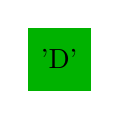
\begin{tikzpicture}[every tree node/.style={draw,circle},
   level distance=1.3cm,sibling distance=.8cm, anchor=west,
    minimum size=8mm,
   edge from parent path={(\tikzparentnode) -- (\tikzchildnode)}]
	\Tree [.\node (A) {} ; 
	  \edge node[auto=right] {\textcolor{blue}{1}};  
	    [.\node (B) {};  
	    \edge node[auto=right] {\textcolor{blue}{1}}; 
	      [.\node[fill=black!30!green] (D) {'A'};  ]
	      \edge node[auto=left] {\textcolor{blue}{0}};  [.\node[fill=black!30!green] (E) {'B'}; ]
	    ]
	  \edge node[auto=left] {\textcolor{blue}{0}};  
	    [.\node (C) {};  
	   	    \edge node[auto=right] {\textcolor{blue}{1}}; 
	   	      [.\node[fill=black!30!green] (F) {'C'};  ]
	   	      \edge node[auto=left] {\textcolor{blue}{0}};  [.\node[fill=black!30!green] (G) {'D'}; ]
	   	    ]]
        \end{tikzpicture}\end{center}
\begin{definition}[Code]\index{Code!Definition}
Ein Code C über den Alphabeten A und B, ist eine Abbildung (= Codierung):
\begin{align}
C: A \rightarrow B
\end{align}
\end{definition}
In unserem Fall ist die Menge $A = \lbrace 00, 01, 10, 11 \rbrace$ und $B = \lbrace$ 'A', 'B', 'C', 'D' $\rbrace$, die Codierung ist folgendermaßen definiert:\\
\begin{enumerate}
\item C(11) = 'A'
\item C(10) = 'B'
\item C(01) = 'C'
\item C(00) = 'D'
\end{enumerate}

Codes, die auf diese Weise gewonnen werden, haben eine wichtige
Eigenschaft --- sie sind präfixfrei.
\begin{definition}[Präfixfrei]\index{Präfixfrei}
Ein Code C mit den Codewörtern $(c_1, c_2 \dots c_n$) heißt präfixfrei oder auch fortlaufende Entzifferbar, wenn kein Codewort $c_i$ präfix eines anderen Codeworts $c_j$ ist.\\
Mit anderen Worten darf kein Codewort am Beginn eines anderen Codeworts stehen.
\end{definition}

Fortlaufende Entzifferbarkeit heißt, dass an jeder Stelle der
codierten Nachricht festgestellt werden kann, ob dort ein Codewort endet,
ohne dass die nachfolgenden Zeichen bekannt sind.

\subsection{Der Huffman-Code}\index{Huffman-Code}
Transformiert man, die Spielestrategie des Huffman-Algorithmus(siehe Definition \ref{def:huffman_algorithmus}) in einen Code, erhält man den \textbf{Huffman-Code}.
Der Huffmancode ist der optimale präfixfreie Code, also der 
mit der kleinsten mittleren Codewortlänge (siehe Definition \ref{def:mittlere_unbestimmtheit}).

\subsection{Der Shannon-Code}\index{Shannon-Code}
Einen anderen Code mit fast optimaler Codewortlänge erhalten wir, wenn
wenn wir von unserer oberen Abschätzung für die Entropie ausgehen. 
Wir wollen also einen Code mit Codewortlängen $l_i=\lceil\log_2(1/p_i)\rceil$
explizit angeben. \\
Dazu ordnen wir die Wahrscheinlichkeiten absteigend
($p_1\ge\dots\ge p_m$) und setzen $f_i=\sum_{j=1}^ip_i$. \\
Das Codewort
$c_i$ erhalten wir, indem wir $f_{i-1}$ als Binaärzahl darstellen und
die ersten $l_i$ Nachkommastellen als Code verwenden. \\
\attention{$f_{i-1}$ ist kleiner als 1, das erste Bit des Codeworts ist also durch $2^{-1}$ bestimmt}

\begin{bsp}[Umwandeln von Dezimal in Binär]:\\\index{Dezimal in Binär}\index{Binär!von Dezimal}
    Wir wollen die Zahl $0{\color{orange}.1}_d$ in eine Binärzahl umwandeln:
    \[0{\color{orange}.1}\cdot 2={\color{blue}0}{\color{red}.2}\;\;\Rightarrow\;\;{\color{blue}0}\]
    \[0{\color{red}.2}\cdot 2={\color{green}0}{\color{brown}.4}\;\;\Rightarrow\;\;{\color{green}0}\]
    \[0{\color{brown}.4}\cdot 2={\color{yellow}0}{\color{gray}.8}\;\;\Rightarrow\;\;{\color{yellow}0}\]
    \[0{\color{gray}.8}\cdot 2={\color{cyan}1}{\color{orange}.6}\;\;\Rightarrow\;\;{\color{cyan}1}\]
    \[0{\color{orange}.6}\cdot 2={\color{blue}1}{\color{red}.2}\;\;\Rightarrow\;\;{\color{blue}1}\]
    \[0{\color{red}.2}\cdot 2={\color{green}0}{\color{brown}.4}\;\;\Rightarrow\;\;{\color{green}0}\]
    \[\vdots\]

Somit lautet die Zahl umgewandelt:
\[0.1_d={\color{blue}0}\overline{{\color{green}0}{\color{yellow}0}{\color{cyan}1}{\color{blue}1}{\color{green}0}}_b
\]
\end{bsp}

Es ist nicht schwer
einzusehen, dass dadurch ein präfixfreier Code definiert wird, der
Shannon-Code. 
Anschaulich lässt sich das Verfahren an einem Beispiel darstellen:

\subsection{Der Fanu-Code}\index{Fanu-Code}
Der einzige Schönheitsfehler dabei ist, dass die Wahrscheinlichkeiten geordnet werden müssen. \\
Diesen Schönheitsfehler behebt der 
Fano-Code.
Hier verwendet man dieselben Notationen wie beim Shannon-Code,
nur codiert man
$\frac{(f_{i-1}+f_i)}{2}$ mit diesmal $\lceil \log_2(\frac{1}{p_i})\rceil+1$ Bits.\\
Wieder mit einem Beispiel:\\

\subsection{Weitere Codierungsverfahren}
Diese Idee kann man auf das Codieren von ganzen Blöcken anwenden, im
Extremfall wird die ganze Nachricht als einzelner Block kodiert. Im 
Vergleich zum Huffman-Code ist das hier möglich, weil nicht der ganze
Code generiert werden muss, sondern nur das eine, das die Nachricht kodiert.
Verahren, die auf dieser Idee beruhen, werden als arithmetische
Codes bezeichnet.

Außer den präfixfreien Codes gibt es auch noch andere, die eindeutig
entziffert werden können. Wir definieren
\begin{definition}\index{entzifferbar!eindeutig (unendlich)|see{eindeutig entzifferbar}}\index{eindeutig entzifferbar}
\begin{enumerate} 
    \item Ein Code heißt endlich \textbf{endlich eindeutig entzifferbar}, wenn
jede endliche Aneinanderreihung von Codewörtern eindeutig in Codewörter
zerlegt werden kann.

\item Ein Code heißt \textbf{eindeutig entzifferbar} (manchmal zur Unterscheidung
    von 1.\ \textbf{unendlich eindeutig entzifferbar}), wenn jede endliche oder
unendliche Aneinanderreihung von Codewörtern eindeutig zerlegt werden kann.
\end{enumerate}
\end{definition}
Der Code $\{0,01\}$ ist offensichtlich nicht präfixfrei, aber trotzdem
eindeutig entzifferbar, für die korrekte Zerlegung muss man allerdings
das nachfolgende Zeichen kennen. Der Code $\{0,01,11\}$ ist endlich
eindeutig entzifferbar, aber nicht eindeutig entzifferbar.

Wir können nun die Frage stellen, ob durch den Verzicht auf die
fortlaufende Entzifferbarkeit etwas gewonnen werden kann, also ob es
einen endlich eindeutig entzifferbaren Code gibt, der kleiner mittlere
Codewortlänge hat als der Huffman-Code. Diese Hoffnung ist allerdings
vergebens, denn es gilt
\begin{satz} Die Codewortlängen in einem endlich eindeutig entzifferbaren
Code erfüllen die Kraft'sche Ungleichung.
\end{satz}
Aus diesem Satz folgt, dass es zu jedem endlich eindeutige entzifferbaren
Code einen präfixfreien Code mit denselben Codewortlängen (und damit
mit derselben mittleren Codewortlänge) gibt.

(universelle Codes)

\index{Codes|)}

\section{Informationsquellen}\index{Informationsquellen|(}
\begin{definition} Eine \textbf{Informationsquelle} \index{Informationsquelle}ist eine Folge
$\mathcal X=(X_1,\dots)$ von Zufallsvariablen.
\end{definition}
Die verschidenen Möglichkeiten für die Abhängigkeitsstruktur dieser
Folge ergeben die Definitionen
\begin{definition}
Wenn die die Zufallsvariablen $X_n$ unabhängig und identisch
verteilt sind, dann heißt $\mathcal X$ \textbf{gedächtnislos}\index{gedächtnislos}.

Wenn $(X_n)$ eine Markovkette bilden oder stationär sind, dann heißt
die Quelle  Markovquelle bzw.\ stationäre Quelle.
Eine irreduzible Markovquelle nennen wir \textbf{ergodisch}\index{ergodisch}.
\end{definition}

Eine wichtige Größe ist die Entropie einer Quelle. Im Sinne der 
der Idee, die wir bei der Einführung der Entropie verwendet haben, 
definieren wir sie über die mittlere Codewortlänge beim optimalen
Kodieren von langen Blöcken:

\begin{definition} Die \textbf{Entropie der Quelle}\index{Entropie!der Quelle}\index{Quelle!Entropie der-|see{Entropie der Quelle}} $\mathcal X$ ist 
\[H(\mathcal X)=\lim_{n\to\infty}{1\over n}H(X_1,\dots,X_n),\]
wenn dieser Grenzwert existiert (wenn nicht, dann hat $\mathcal X$
keine Entropie.)
\end{definition}

Für eine gedächtnislose Quelle gilt
\[H(\mathcal X)=H(X_1).\]
Für eine (irreduzible) Markovquelle mit Übergangsmatrix $P$ ergibt sich
\[H(X)=\sum\pi_iH(P_i),\]
wobei $P_i$ die $i$-te Zeile von $P$ und $\pi$ die stationäre Verteilung ist.

Für eine stationäre  Quelle existiert die Entropie.

\begin{satz}[Shannon-MacMillan] Für eine stationäre Quelle gilt
\[\lim_{n\to\infty}{1\over n}\log_2 p(X_1,\dots,X_n)=-nH(\mathcal X)\]
in Wahrscheinlichkeit.
\end{satz}
Das kann man so sehen, dass mit hoher Wahrscheinlichkeit gilt, dass die 
Wahrscheinlichkeit, genau die Folge $(X_1,\dots,X_n)$ zu ziehen
$\approx 2^{-nH(\mathcal X)}$ ist.

\index{Informationsquellen|)}
\section{Blockcodes}
\section{Kanalcodierung}
\section{Natürliche Sprachen als Informationsquellen}
\index{Informationstheorie|)}
